\documentclass[runningheads,a4paper]{llncs}

\usepackage[T1]{fontenc}
\usepackage{amsmath,amssymb}
\usepackage{graphicx}
\usepackage{booktabs}
\usepackage{array}
\usepackage{multirow}
\usepackage{tikz}
\usetikzlibrary{arrows.meta,positioning,fit,backgrounds}
\usepackage{xcolor}
\usepackage{cite}
\usepackage[hidelinks]{hyperref}

\graphicspath{{figures/}}
% generated by make_tables.py - do not edit
\newcommand{\AsixClosed}{0.582}
\newcommand{\AsixRaw}{0.398}
\newcommand{\BsixClosed}{0.386}
\newcommand{\BsixRaw}{0.287}
\newcommand{\AlabClosed}{0.572}
\newcommand{\AlabRaw}{0.378}
\newcommand{\BlabClosed}{0.546}
\newcommand{\BlabRaw}{0.378}
\newcommand{\AboxClosed}{0.532}
\newcommand{\BboxClosed}{0.349}
\newcommand{\AsingleClosed}{0.298}
\newcommand{\BsingleClosed}{0.254}
\newcommand{\Acars}{20}
\newcommand{\Bcars}{7}
\newcommand{\AsixVClosed}{0.565}
\newcommand{\BsixVClosed}{0.372}
\newcommand{\Acentre}{1.1}
\newcommand{\Bcentre}{2.6}
\newcommand{\Aalong}{0.96}
\newcommand{\Aacross}{0.27}
\newcommand{\Balong}{2.5}
\newcommand{\Bacross}{0.31}
\newcommand{\Acommon}{17}
\newcommand{\Bcommon}{6}
\newcommand{\Egopath}{13\,\%}
\newcommand{\Egolabels}{187}
\newcommand{\Egofound}{25}
\newcommand{\Egorecall}{0.13}
\newcommand{\Egoprecision}{0.53}

% generated by make_tables.py - do not edit
\newcommand{\DairCars}{109}
\newcommand{\DairClips}{20}
\newcommand{\DairSites}{7}
\newcommand{\DairFrames}{2950}
\newcommand{\DairOursRaw}{0.463}
\newcommand{\DairBoxRaw}{0.465}
\newcommand{\DairOursClosed}{0.612}
\newcommand{\DairBoxClosed}{0.618}
\newcommand{\DairAlong}{1.44}
\newcommand{\DairAcross}{0.59}
\newcommand{\SpdCars}{104}
\newcommand{\SpdClips}{12}
\newcommand{\SpdSites}{6}
\newcommand{\SpdFrames}{2733}
\newcommand{\SpdOursRaw}{0.450}
\newcommand{\SpdBoxRaw}{0.488}
\newcommand{\SpdOursClosed}{0.618}
\newcommand{\SpdBoxClosed}{0.636}
\newcommand{\SpdAlong}{1.37}
\newcommand{\SpdAcross}{0.29}


\newcommand{\R}{\mathbb{R}}
\newcommand{\vect}[1]{\mathbf{#1}}

\begin{document}

\title{Learning-Free 3D Car Shapes from a Single Roadside Video}
\titlerunning{Learning-Free 3D Car Shapes from a Roadside Video}
\author{Dmitriy Zhuravlev}
\authorrunning{D. Zhuravlev}
\institute{T. Shevchenko National University, Kyiv, Ukraine\\
\email{dzhuravlev@ukr.net}}

\maketitle

\begin{abstract}
Roadside cameras watch the same intersection for years, yet monocular 3D perception for them is almost always a
learned detector that outputs boxes and needs thousands of labelled 3D boxes from the same kind of camera. We show
that the 3D \emph{shape} of the cars that pass a fixed, calibrated camera can be recovered without any learning and
without labels. In short windows of the video every moving car is triangulated and its planar rigid motion and the
depth of every vertex are solved jointly; the windows of one car are then solved together as one rigid car, with one
pose per frame shared by all its windows, mirrored about the car's symmetry plane, averaged as a robust height field
and completed by a visual hull of edge-snapped silhouettes; a car whose length was never seen across the viewing ray
takes the length and profile of its body type. LiDAR and 3D labels are used for evaluation only; labelled 2D boxes
serve once, as the tracker of a diagnostic experiment on pedestrians. Against the cars' accumulated LiDAR, completed by
its mirror image, the models reach a solid (height-field) IoU of \AsixClosed{} on the intersection on which the method
was tuned (labelled boxes: \AlabClosed{}) and \BsixClosed{} on a second intersection (\BlabClosed{}). Unchanged, they
reach \DairOursClosed{} on \DairCars{} cars of DAIR-V2X-C and \SpdOursClosed{} on \SpdCars{} cars of V2X-Seq-SPD,
statistically level with the labelled 3D boxes scored the same way (\DairBoxClosed{} and \SpdBoxClosed{}), also on
the clips that informed no design choice. From
silhouettes alone, nearby pedestrians and cyclists get coarse models when they are tracked well. We also show that the
usual LiDAR reference is strongly biased at long range: against the raw accumulated scan the labelled box itself
scores only \AlabRaw{}. Finally, the same pipeline on a moving vehicle camera with monocular visual odometry finds
only a small share of the cars: the method depends on a fixed, elevated viewpoint.
\keywords{3D reconstruction \and vehicle shape \and roadside camera \and visual hull \and structure from motion \and
learning-free}
\end{abstract}

% ------------------------------------------------------------------------------------------------------------------
\section{Introduction}

Cameras mounted on poles at intersections see every car from a high, fixed viewpoint and for a long time. Monocular
3D perception for such cameras is dominated by learned detectors that regress a 3D box per object
\cite{rope3d,bevheight}, trained on large labelled datasets such as Rope3D \cite{rope3d}, DAIR-V2X \cite{dairv2x}
and V2X-Seq \cite{v2xseq}. A box carries position, size and heading, but not the shape of the car, and a detector
trained for one camera height and one city degrades when either changes.

A fixed camera offers something a single image does not: every car is seen in many frames, from a slowly changing
direction, against a background that does not move. This is the classical setting of structure from motion for
rigidly moving objects \cite{ozden2010} and of shape from silhouettes \cite{laurentini,spacecarving}. This paper
asks how far these classical tools go today for full car shapes at up to 70~m from the camera, and measures the
answer against LiDAR.

Our earlier work recovered 3D boxes from a single image with inverse perspective mapping (IPM) \cite{lift,efficient_orig}
and segmented moving objects by optical-flow clustering \cite{moving_orig}. Here we go from boxes to shapes and from
single frames to the whole video. The contributions are:
\begin{enumerate}
\item a learning-free reconstruction of every moving car in short windows: a dense triangulation of the car body,
  tracked through the window, with the planar rigid motion of the car and the depth of every vertex along its viewing
  ray solved jointly under road-contact, smoothness and non-holonomic constraints (Sect.~\ref{sec:window});
\item a video-level fusion per car: all windows of a car solved together as one rigid car (one pose per frame shared
  by every window), the symmetry plane, a weighted-median height field over all windows, a visual hull of silhouettes
  snapped to image edges for the cabin, and the body type's length and profile only where the video never measured
  them (Sect.~\ref{sec:fusion});
\item an evaluation against accumulated LiDAR that exposes a large bias of the raw reference at long range and
  corrects it, with the labelled boxes scored the same way as an upper reference (Sect.~\ref{sec:protocol});
\item experiments on the intersections of two datasets and on a moving vehicle camera, an ablation, paired
  confidence intervals against the labelled boxes, and a direct account of where the method fails
  (Sects.~\ref{sec:results}--\ref{sec:limits}).
\end{enumerate}

% ------------------------------------------------------------------------------------------------------------------
\section{Related Work}

\paragraph{Monocular 3D detection.} Geometry-aware detectors fit a 3D box to a 2D detection
\cite{deep3dbox}; keypoint and centre-based networks regress boxes directly \cite{smoke,monodle,monoflex,gupnet,fcos3d};
others predict depth first \cite{pseudolidar,caddn} or lift image features to a bird's-eye view \cite{bevdet,bevdepth}.
For roadside cameras, BEVHeight \cite{bevheight} regresses the height above the ground instead of depth, which suits
the high viewpoint; Rope3D \cite{rope3d}, DAIR-V2X \cite{dairv2x} and V2X-Seq \cite{v2xseq} provide the benchmarks.
All of these are trained with 3D boxes and output boxes. Classical traffic-camera work calibrates the camera from
vanishing points \cite{dubska_diamond_space,sochor}, segments and tracks vehicles from motion \cite{kanhere} and lifts
2D detections with IPM \cite{mallot,lift,efficient_orig}.

\paragraph{Vehicle shape.} Learned category models fit a deformable car shape to a single image
\cite{kar2015,deepmanta,rcnn3d} or to stereo street scenes \cite{engelmann2016}; they need a shape prior learned from
CAD models or 3D annotations. Multibody structure from motion reconstructs several rigidly moving objects from point
tracks \cite{ozden2010}, and dense methods reconstruct dynamic scenes from two frames \cite{kumar2017}; bundle
adjustment \cite{bundleadj} refines both. Shape from silhouettes bounds an object by the intersection of its viewing
cones, the visual hull \cite{laurentini}, refined by photo-consistency in space carving \cite{spacecarving}.

\paragraph{This work} combines these classical parts for a fixed roadside camera: motion and per-vertex depth for the
visible body, silhouettes for the cabin, symmetry and the whole video for the hidden side, and no learned component
anywhere in the reconstruction.

% ------------------------------------------------------------------------------------------------------------------
\section{Setting}\label{sec:setting}

The camera is fixed and calibrated: a world point $\vect{X}$ projects to $\pi(\vect{X}) \sim \vect{K}(\vect{R}\vect{X} +
\vect{t})$. The world frame has the road as the plane $z = 0$; its height and tilt relative to the camera are fitted
once (a single plane fit, equivalent to measuring the camera's height and tilt). A pixel $\vect{u}$ defines the ray
$\vect{X}(s) = \vect{C} + s\,\vect{d}(\vect{u})$ from the camera centre $\vect{C}$; its intersection with the road
is the inverse perspective mapping (IPM) \cite{mallot}. Cars move rigidly on the road plane: a point $\vect{X}$ of a
car moves from the reference frame to frame $j$ as
\begin{equation}
  \mathcal{M}_j(\vect{X}) = \begin{pmatrix} \vect{R}(\theta_j)(\vect{X}_{xy} - \vect{c}) + \vect{c} + \vect{t}_j \\ X_z \end{pmatrix},
  \label{eq:motion}
\end{equation}
with yaw change $\theta_j$, translation $\vect{t}_j \in \R^2$ and the car's centre $\vect{c}$ on the road.

% ------------------------------------------------------------------------------------------------------------------
\section{Method}

Figure~\ref{fig:pipeline} shows the pipeline, Fig.~\ref{fig:overview} the first steps on one frame and
Fig.~\ref{fig:steps} a car from its triangulation to its model.

\begin{figure}[t]
\centering
\resizebox{\textwidth}{!}{%
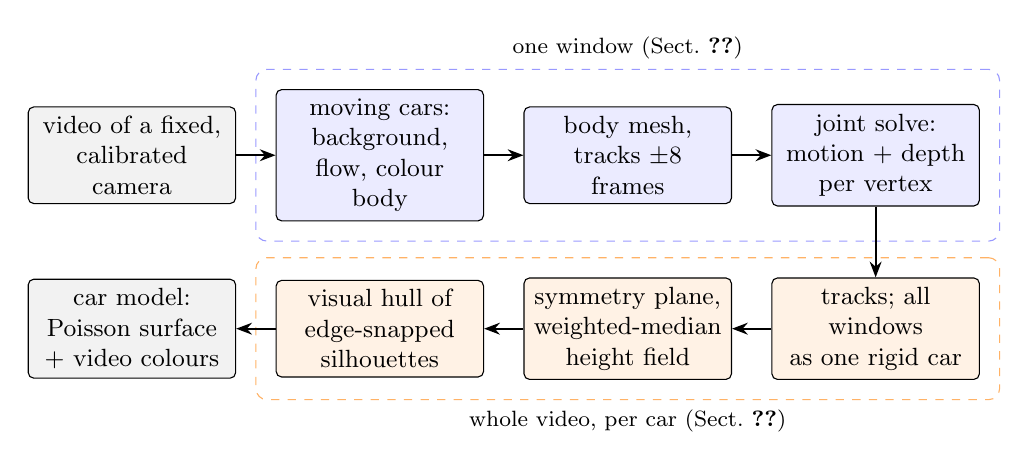
\begin{tikzpicture}[node distance=4mm and 5mm, every node/.style={font=\small},
  box/.style={draw, rounded corners=2pt, align=center, minimum height=11mm, text width=24mm, fill=#1},
  box/.default=white, arr/.style={-{Stealth[length=2mm]}, thick}]
  \node[box=gray!10] (video) {video of a fixed,\\ calibrated camera};
  \node[box=blue!8, right=of video] (seg) {moving cars:\\ background,\\ flow, colour body};
  \node[box=blue!8, right=of seg] (mesh) {body mesh,\\ tracks $\pm 8$ frames};
  \node[box=blue!8, right=of mesh] (solve) {joint solve:\\ motion + depth\\ per vertex};
  \node[box=orange!10, below=9mm of solve] (track) {tracks; all windows\\ as one rigid car};
  \node[box=orange!10, left=of track] (sym) {symmetry plane,\\ weighted-median\\ height field};
  \node[box=orange!10, left=of sym] (hull) {visual hull of\\ edge-snapped\\ silhouettes};
  \node[box=gray!10, left=of hull] (model) {car model:\\ Poisson surface\\ + video colours};
  \draw[arr] (video) -- (seg); \draw[arr] (seg) -- (mesh); \draw[arr] (mesh) -- (solve);
  \draw[arr] (solve) -- (track); \draw[arr] (track) -- (sym); \draw[arr] (sym) -- (hull); \draw[arr] (hull) -- (model);
  \begin{scope}[on background layer]
    \node[draw=blue!40, dashed, rounded corners, fit=(seg)(mesh)(solve), inner sep=2.5mm, label={[font=\footnotesize]above:one window (Sect.~\ref{sec:window})}] {};
    \node[draw=orange!60, dashed, rounded corners, fit=(track)(sym)(hull), inner sep=2.5mm, label={[font=\footnotesize]below:whole video, per car (Sect.~\ref{sec:fusion})}] {};
  \end{scope}
\end{tikzpicture}}
\caption{The pipeline. Every window of $\pm 8$ frames is reconstructed on its own (blue); the windows of one car are
then fused over the whole video (orange). No step is learned; LiDAR and 3D labels are used only to evaluate.}
\label{fig:pipeline}
\end{figure}

\begin{figure}[t]
\centering
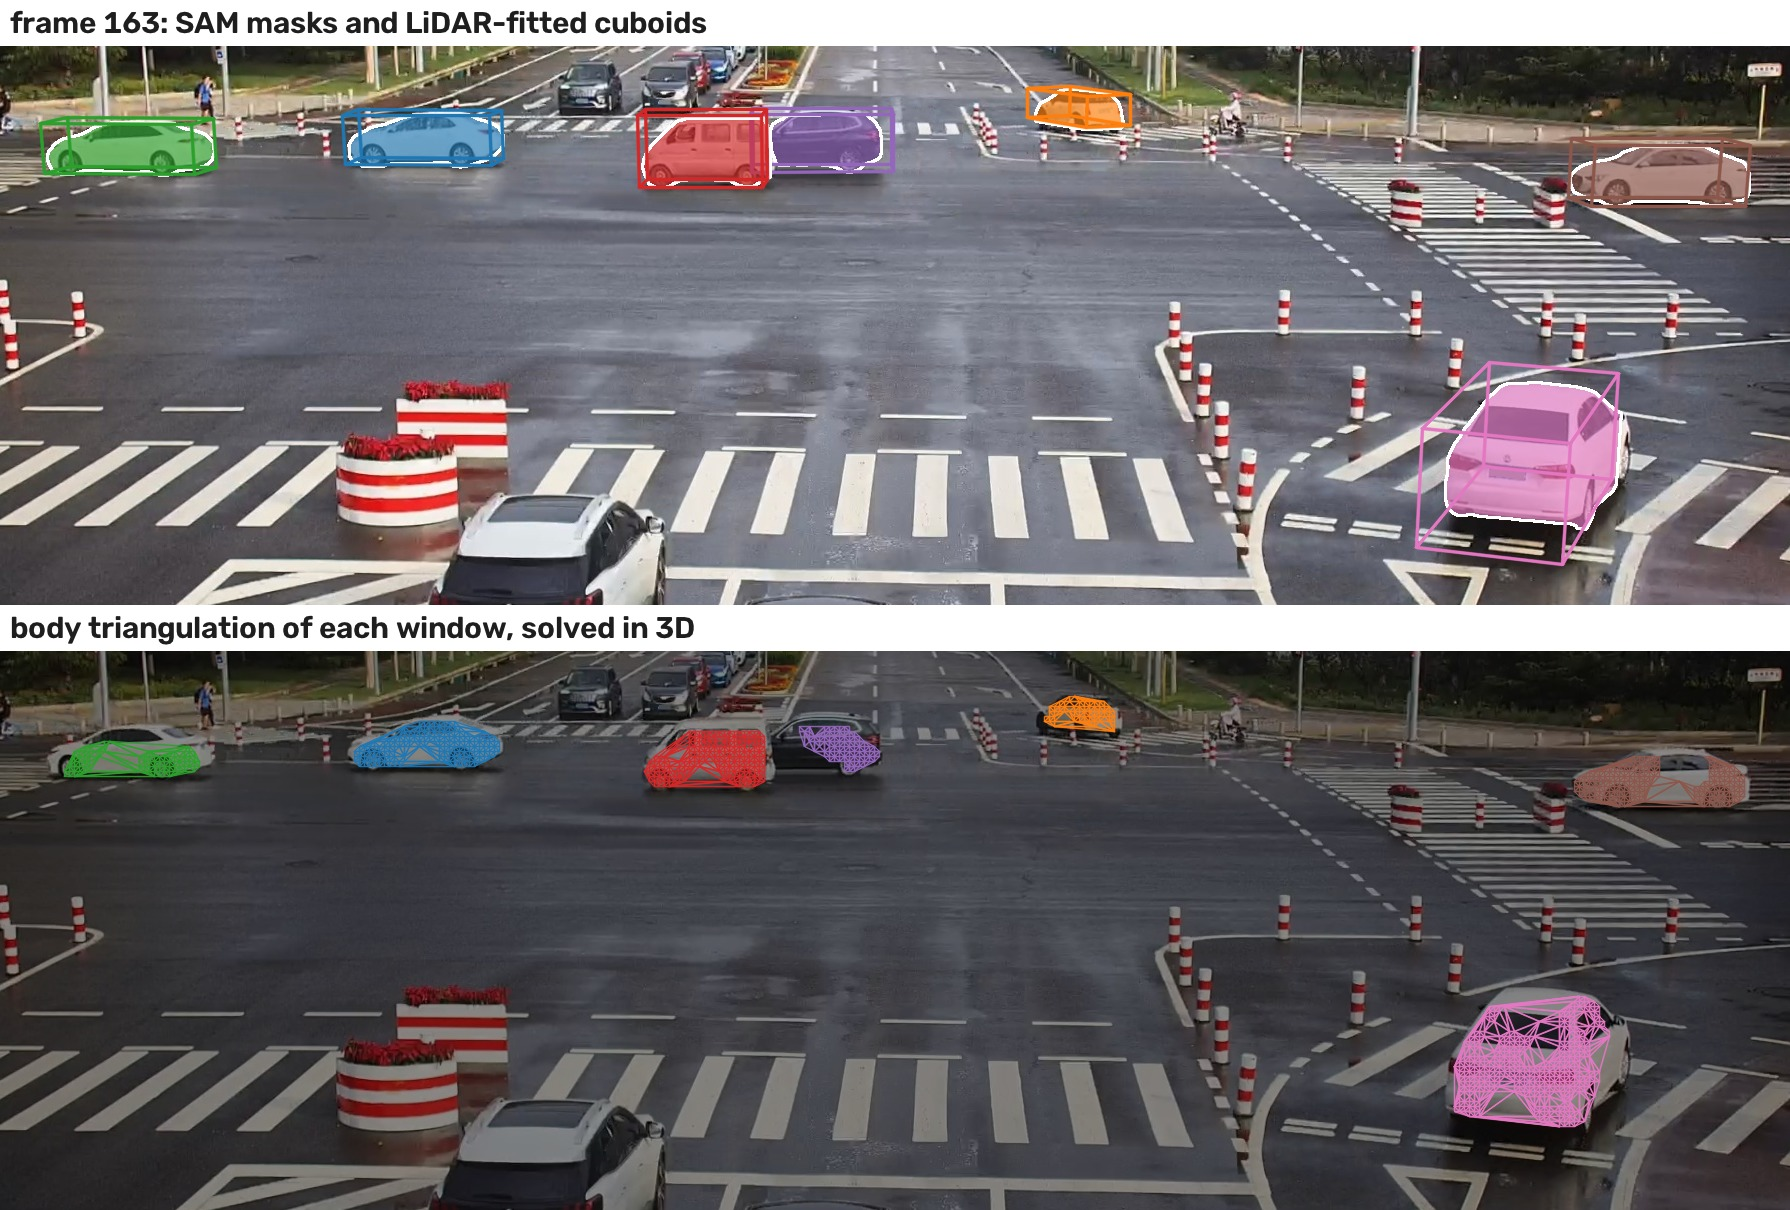
\includegraphics[width=\textwidth]{window.jpg}
\caption{One frame of intersection~A. Top: the moving cars' SAM masks (white outline) and their LiDAR-fitted
cuboids. Bottom: the body triangulation of every window whose reference frame this is, one colour per car, each
solved in 3D.}
\label{fig:overview}
\end{figure}

\subsection{One window: motion and depth of the visible body}\label{sec:window}

\paragraph{Moving cars.} The background is the per-pixel median of the video. A frame's foreground blobs are cut at
the contact line below which the wet road mirrors the car, split into separate cars by clustering the optical flow
\cite{farneback,moving_orig}, and freed of the cast shadow by a brightness/saturation test. Blobs whose mean flow is
below $1.5$~px per frame are stopped cars and are skipped: without motion there is no parallax.

\paragraph{The body and its mesh.} Inside each blob the pixels are clustered by colour ($k$-means with $k = 3$
in CIE Lab); the largest cluster and the clusters within $\Delta E \le 20$ of it form the \emph{body}: the painted
metal without tyres, dark trims and shadow, whose texture moves rigidly with the car. The body receives a dense set of vertices --- Shi--Tomasi corners
\cite{shitomasi}, a regular grid of at most 5~px (at least 400 vertices per body) and points 2~px inside its
outline --- and is triangulated by
Delaunay. Every vertex is tracked through the window of $\pm 8$ frames with pyramidal Lucas--Kanade \cite{lucas_kanade}
and a forward--backward check; long tracks of near, fast cars are cut at 100~px of image motion.

\paragraph{Joint solve.} The unknowns are the motion $\vect{m}_j = (\theta_j, \vect{t}_j)$ of the car in every frame
of the window ($\vect{m}_r = 0$ in the reference frame $r$) and the depth $s_i$ of every vertex along its reference
ray, $\vect{X}_i = \vect{C} + s_i \vect{d}_i$. They minimise
\begin{align}
  E = &\sum_{i,j} \big\| \pi_j\big(\mathcal{M}_j(\vect{X}_i)\big) - \vect{u}_{ij} \big\|^2
      + \lambda \sum_{(a,b)} w_{ab} \|\vect{n}_a - \vect{n}_b\|^2
      + W_a \sum_{i \in \mathcal{L}} (X_{i,z} - h_r)^2 \nonumber\\
      &+ W_m \sum_j \|\vect{m}_{j-1} - 2\vect{m}_j + \vect{m}_{j+1}\|^2_{\Sigma}
      + W_h \sum_j \big( \vect{u}^\perp \cdot \vect{R}(-\bar\theta_j)(\vect{t}_{j+1} - \vect{t}_j) \big)^2 .
  \label{eq:energy}
\end{align}
with every squared residual $r^2$ entering through the robust soft-$\ell_1$ loss $\rho(r^2) = 2(\sqrt{1 + r^2} - 1)$,
which grows only linearly for large residuals. The first term is the reprojection error of the tracked vertices. The
second makes the normals $\vect{n}_a,
\vect{n}_b$ of triangles sharing an edge agree, with weight $w_{ab} = 1$ inside a colour region and $0.3$ across a
colour edge, so that panels stay smooth and creases follow paint and trim lines. The third places the body's lower
edge on its height above the road, $h_r$ (set below): $\mathcal{L}$ holds the lowest vertex in each of 8 slices along the body,
so that the edge is anchored along its whole length and not at one end; this anchor fixes the scale. The fourth is
temporal smoothness of the motion, with $\|\vect{m}\|^2_{\Sigma} = (8\,\text{m}\cdot\theta)^2 + \|\vect{t}\|^2$, so that
one radian of yaw weighs like 8~m of translation; the fifth forbids a sideways step: a car moves along its heading ($\vect{u}^\perp$
is the normal of the initial direction of travel, $\bar\theta_j$ the mean yaw of the step). Both motion priors are
divided by the length of the path, so that they do not favour a smaller copy of the car closer to the camera, which
would move less. Every vertex is bounded to $0 \le z \le 3.2$~m and the lower-edge vertices to $h_r \pm 0.1$~m.

The motion is initialised by a RANSAC Procrustes fit \cite{fischler_bolles_ransac} of the IPM points of the lowest
vertices, frame to frame, smoothed by a quadratic in time; the yaw change follows the direction of the path. The
depths start at the intersection of each vertex's rays under that motion. After the solve, vertices whose residual
exceeds $\max(1.5~\text{px}, 2.5 \times \text{median})$ --- background dragged along by the tracker at the outline,
or another car --- are removed and the solve is repeated (two rounds).

The body height $h_r$ is $0.45$~m in a first pass over the video; the second pass uses the value of each car's body
type from the first pass's models (sedan and hatchback $0.40$, SUV $0.52$, van $0.48$~m).

\subsection{The whole video: one model per car}\label{sec:fusion}

\paragraph{Tracks.} Windows are reconstructed every second frame. The cars of successive windows are linked by the
Hungarian method \cite{kuhn} on their road positions, predicted with their solved velocity, inside a gate of
$2.5~\text{m} + 4\,\%$ of the range; tracks of fewer than 5 windows are dropped.

\paragraph{One rigid car per track.} Each window has solved its own motion, so two windows of the same car disagree
on where the car is when they overlap in time. We therefore solve all windows of a track together, as rigid structure
from motion of one moving object \cite{ozden2010}: one planar pose $\vect{Q}_g = (\phi_g, \vect{p}_g)$ of the car per
frame $g$, shared by every window that sees frame $g$, and the depths of all windows' vertices. A vertex of window $w$,
a point $\vect{X}$ in the world at the window's reference frame $r_w$, is at
$\vect{R}(\phi_g - \phi_{r_w})(\vect{X}_{xy} - \vect{p}_{r_w}) + \vect{p}_g$ in frame $g$. The energy is that of
Eq.~(\ref{eq:energy}) summed over the windows --- reprojection, surface smoothness and the body-edge anchors of every
window --- with the motion terms on the shared poses of the whole track; one pose is held fixed, which removes the
gauge freedom (a common planar motion of all poses and points). The solve starts from a chain: the middle window's pose comes from the
smoothed path of the track, and each window places the reference frame of its neighbour through its own solved
motion, so that the start agrees with every window's points (0.3--0.5~px). The vertices on the outline of a window's
triangulation are left out: the tracker follows the moving edge of the car's mask there, not a point of its surface,
and with them the track solve stretches the cars by 0.5~m. Every window then enters the car frame ($x$ forward, $y$
left, $z$ up) through the shared pose of its reference frame, with no further alignment. Before this step, the windows
were aligned to each other by a trimmed planar ICP \cite{icp}; along the car's own axis the point cloud is
self-similar, and the alignment slid.

\paragraph{Heading and the car's box.} The orientation of a car is never fitted to its shape; it comes from its
motion. In a window, the yaw changes $\theta_j$ are unknowns of Eq.~(\ref{eq:energy}), started from a RANSAC
Procrustes fit of the lowest vertices; the window's velocity is the solved translation per frame. Over the track,
these velocities are smoothed by a quadratic in time, and the heading of each window is the direction of the smoothed
velocity (the tangent of the smoothed path of the footprint where the car barely moves, below 5~cm per frame). This
heading starts the track solve, whose pose $\vect{Q}_g = (\phi_g, \vect{p}_g)$ then gives the car's heading
$\phi_g$ in every frame; the fifth term of Eq.~(\ref{eq:energy}) keeps it along the direction of travel. The car
frame has its $x$ axis along $\phi_g$, and the model is built in it, so the car's bounding box is aligned with the
heading: its length and width are the extents of the occupied height-field columns along $x$ and $y$, its height the
98th percentile of the column heights. A car that turns is therefore boxed along its momentary direction of travel.

\paragraph{Symmetry.} The symmetry plane $y = y_0$ maximises the share of points whose mirror image has a neighbour
within 12~cm \cite{mitra2006}; the points are re-centred on it and used together with their mirror images, which
gives the unseen side of the car. Points beyond the widest car ($\pm 1.05$~m) are dropped.

\paragraph{Height field.} In every 10~cm column of the car frame each window contributes the height of its highest
point. The model height is the weighted median over the windows that saw the column, with weights
$1 / (0.5 + e_k)$ from each window's reprojection error $e_k$ in pixels, and at least $\max(2, 0.2 N)$ of the $N$
windows must see a column. Columns whose point density is below $25\,\%$ of the densest column of the same
cross-section are dropped: the true surface collects points from every window, the along-ray depth noise spreads
them thin. A $3 \times 3$ median filter and the largest connected component finish the field.

\paragraph{Cabin from silhouettes.} The body field covers the painted body; windows and roof are often too dark or
too uniform to track. The full silhouette of the car in every window --- background subtraction with the reflection
and the shadow removed --- is snapped to the image edges: every contour point moves up to $\pm 3$~px along its normal
to the strongest gradient, as an active contour would \cite{snakes}. Voxels of 10~cm are kept if they, and their
mirror images, project inside the silhouette in at least $95\,\%$ of the windows that see them (a visual hull
\cite{laurentini}; $80\,\%$ for a car whose length is bounded by the prior, below, where the strict vote only cuts
away volume); the top of the kept voxels is the cabin field, and the model is the higher of the body and cabin
fields. A high camera sees a car from nearly the same direction in all windows, so the cone of one silhouette is
long along the viewing ray and rises toward the camera; the hull is therefore capped at $1.9$~m. For cars nearer than
40~m the silhouettes alone are used.

\paragraph{Body type, width and length.} The side profile of the car's silhouette in its most side-on windows gives
scale-free features (length to height, share of the length under the roof, height of the front and rear fifths) and
a type by fixed rules: sedan, hatchback, SUV or van. For a car seen from the side the width lies nearly along the viewing ray, where a single camera measures it worst; the width is therefore bounded by the type's typical width
(sedan 1.90, hatchback 1.85, SUV 1.95, van 2.05~m). The length is measured only where the car is seen side-on: a
window with $|\sin(\text{heading} - \text{viewing ray})| \ge 0.5$ sees the length across the ray. A car seen side-on in
fewer than two windows --- most often a car seen only from behind --- has a length the video never measured:
it is cut to 4.6~m at its camera end, where the silhouette cone smears, and its heights become its body type's
profile, a box up to the shoulder line and a cabin box on top with a sloping windshield and rear window (0.9 and
0.6~m long). These are priors, not measurements, and we report the two groups of cars separately
(Sect.~\ref{sec:results}). Cars measured side-on, vans included, keep their own length and shape.

\paragraph{Mesh and colour.} The height field is regularised between its raw surface and a convex hull: every
cross-section of the car becomes its upper concave envelope, which fills notches and holes in the roof, while along
the car narrow spikes and thin sheets are removed (grey-scale opening with a 0.3~m structuring element) and dips
narrower than 0.7~m are filled (grey-scale closing with a 0.7~m structuring element), so that the steps from bonnet to windshield to roof survive; a Gaussian of 1.2 cells follows. The
surface of the regularised field (marching cubes \cite{marchingcubes}) is finally replaced by its Poisson surface
\cite{kazhdan2006} on a 6~cm grid, which removes the staircase of the 10~cm columns; this changes the shown model, not
the height field that is evaluated. Every vertex takes the original pixel, sampled bilinearly, of the windows that see
it best --- preferring views with a larger cosine between its normal and the viewing direction and nearer views (the
cosine divided by the distance) --- where it
faces the camera, lies inside the car's silhouette and is not hidden by another part of the model (a z-buffer of the
model's own vertices): of its five best views the medoid pixel is kept, so that one view whose pose is a little off
is outvoted. Before sampling a view, the model's projected outline is shifted onto that window's silhouette (the best
overlap within 48~px), and the view is weighted by that overlap: the windows at the ends of a track are often off by
tens of pixels, and without this the glass lands on the bonnet. A vertex and its mirror image take the better seen of
the two. A vertex no window sees takes, near a seen vertex (0.3~m), that vertex's colour; farther, below the belt line
one body colour, the median of the seen vertices between 30\,\% of the height and the belt line, and above it the
median colour of the seen vertices at the same height --- glass at window height, paint on the roof.

% ------------------------------------------------------------------------------------------------------------------
\section{Evaluation Protocol}\label{sec:protocol}

\paragraph{Data.} \emph{Intersection A} is the infrastructure side of the V2X-Seq-SPD example \cite{v2xseq}
(sequence 0058, 251 frames at 10~Hz, $1920 \times 1080$, camera 8.45~m above the road and tilted $15^\circ$ down,
wet road). \emph{Intersection B} is the infrastructure side of the DAIR-V2X-C example \cite{dairv2x} (84 frames at
12.5~Hz, camera 8.96~m high, dry road); its labels have no track identities, so we link the labelled boxes from frame
to frame (for evaluation only). \emph{The moving camera} is the vehicle side of the same V2X-Seq sequence (250 frames,
camera 1.7~m above the road). The parameters were chosen on intersection A, but B and five clips of the larger
evaluation (Sect.~\ref{sec:results}) informed three design choices: the length cap only for cars never seen side-on,
rather than for every car, was chosen on A, B and those five clips; the softer hull vote for those cars was chosen on A and B;
and the joint solve of a track was adopted after it improved A, B and one of the five clips. Ideas that did not help
on A and B were dropped. B is therefore not a clean hold-out; for the larger evaluation we also report the clips that
informed no choice.

\paragraph{LiDAR reference.} For each labelled car the LiDAR points inside its box are collected over its whole track
in the box frame, mirrored about the box's vertical centre plane along its heading and turned into a height field of
5~cm columns. This \emph{symmetry-completed} reference fills the side the LiDAR did not see; it favours symmetric
shapes, but our models and the labelled boxes are both symmetric, so it favours neither over the other. A car is
evaluated when its reference holds more than 200 points and when one of our tracks is matched to it: our car centre
is within 3~m of the labelled centre (5~m on B, see Sect.~\ref{sec:results}) in at least half of its windows.

\paragraph{The reference is biased.} At 60~m a LiDAR scan is sparse: the accumulated points leave gaps between scan
lines on the roof and the bonnet, and these gaps are counted as empty space. Scored against the raw field, the
\emph{labelled box itself} reaches a mean solid IoU of only \AlabRaw{} on intersection A --- about what our models
score --- so the raw reference cannot rank methods near the top. We close the gaps by a grey-scale closing of the
height field with a radius of 15~cm, which fills gaps between returns but does not extend the outline; against the
closed field the labelled box scores \AlabClosed{} on A and \BlabClosed{} on B. We report both references.
Figure~\ref{fig:lidar} shows the effect for two cars.

\begin{figure}[t]
\centering
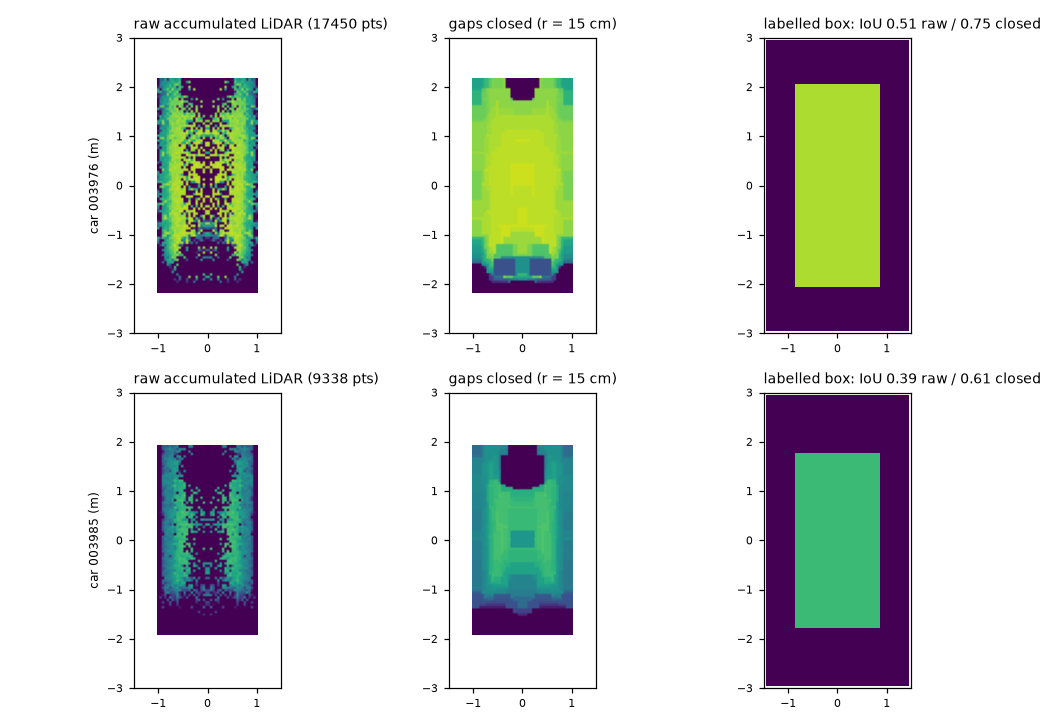
\includegraphics[width=0.85\textwidth]{lidar_reference.png}
\caption{The LiDAR reference of two cars of intersection A in the car frame (colour: height, 0--2~m). The raw
accumulated field has gaps between the scan lines (left); closed with a radius of 15~cm it keeps the outline
(middle). The labelled box (right) scores far lower against the raw field than against the closed one.}
\label{fig:lidar}
\end{figure}

\paragraph{Metrics.} Both height fields are centred on their footprints and compared with both headings. The
\emph{solid IoU} is $\sum \min(H, L) / \sum \max(H, L)$ over all columns, for our height field $H$ and the reference
$L$, on a grid that covers both, so that a model longer or wider than the car is penalised; the \emph{footprint IoU}
compares the occupied columns; the \emph{height error} is the median $|H - L|$ over columns occupied in both. Length, width and height are compared with the labelled box. As a check that the closing does not favour
smooth models, the \emph{scanned IoU} leaves out only the reference volume the closing invented (columns without a
return in the raw field), keeping every other column, so that a model sticking out of the car still counts. Paired
differences between our models and the labelled boxes on the same cars are given with 95\,\% bootstrap intervals
(5000 resamples); a label our tracker split into two track fragments keeps the longer one.

% ------------------------------------------------------------------------------------------------------------------
\section{Results}\label{sec:results}

\begin{table}[t]
\centering
\caption{Cars against their accumulated LiDAR (mean over the evaluated cars). IoU against the raw and the gap-closed reference, footprint IoU and height error against the closed one, size errors against the labelled box. The labelled box and a box of our own estimated size are scored in the same way.}
\label{tab:main}
\setlength{\tabcolsep}{4pt}
\resizebox{\textwidth}{!}{%
\begin{tabular}{llccccccc}
\toprule
 & & \multicolumn{2}{c}{solid IoU} & footprint & height & \multicolumn{3}{c}{size error (m)} \\
\cmidrule(lr){3-4}\cmidrule(lr){7-9}
 & & raw & closed & IoU & err.\ (cm) & $L$ & $W$ & $H$ \\
\midrule
\multirow{4}{*}{A (20 cars)} & labelled box & 0.384 & 0.581 & 0.691 & -- & 0 & 0 & 0 \\
 & box of our size & 0.353 & 0.569 & -- & -- & 0.58 & 0.15 & 0.34 \\
 & best single window & 0.239 & 0.301 & -- & -- & -- & -- & -- \\
 & \textbf{ours} & \textbf{0.414} & \textbf{0.608} & 0.724 & 25.6 & 0.58 & 0.15 & 0.34 \\
\midrule
\multirow{4}{*}{B (7 cars)} & labelled box & 0.380 & 0.550 & 0.693 & -- & 0 & 0 & 0 \\
 & box of our size & 0.327 & 0.485 & -- & -- & 2.27 & 0.19 & 0.27 \\
 & best single window & 0.228 & 0.272 & -- & -- & -- & -- & -- \\
 & \textbf{ours} & \textbf{0.372} & \textbf{0.492} & 0.577 & 27.1 & 2.27 & 0.19 & 0.27 \\
\bottomrule
\end{tabular}}
\end{table}


\paragraph{Intersection A (tuning set).} Table~\ref{tab:main} compares the models with three references scored in
the same way: the labelled box, a box of our own estimated length, width and height, and the best single window
without averaging and symmetry. A has 19 tracks of 18 cars: the tracker split one car in two, and each track is
scored. A is the intersection on which the method was tuned, so its comparison with the labelled box is in-sample; B
and the larger evaluation below informed only the few choices listed in Sect.~\ref{sec:protocol}. Against the closed reference our models reach
\AsixClosed{}, above the labelled boxes (\AlabClosed{}) and above a box of the same size as ours (\AboxClosed{}): the
shape adds to the dimensions. A single window reaches only \AsingleClosed{}; the gain comes from fusing the video
(Fig.~\ref{fig:steps}). Figure~\ref{fig:scene} draws the models back into one frame of the video and
Fig.~\ref{fig:cars} shows the best cars up close with their LiDAR.

\begin{table}[t]
\centering
\caption{Paired difference of the mean solid IoU (ours $-$ labelled box) against the gap-closed LiDAR, per car, with a 95\,\% bootstrap confidence interval (5000 resamples, fixed seed). \emph{measured}: the car's length was seen side-on ($\ge 2$ side-on windows); \emph{completed}: never seen side-on, length and profile completed from its cuboid; \emph{held-out}: without the five clips that informed a choice during development. Intersection A is the tuning set of the method; B informed three choices (Sect.~\ref{sec:protocol}).}
\label{tab:paired}
\small
\begin{tabular}{llrcl}
\toprule
Dataset & length & cars & mean $\Delta$ IoU & 95\,\% CI \\
\midrule
intersection A (tuning) & all & 24 & +0.092 & [+0.070, +0.115] \\
 & measured & 22 & +0.092 & [+0.070, +0.116] \\
 & completed & 2 & +0.089 & [+0.031, +0.146] \\
\midrule
intersection B & all & 15 & +0.107 & [+0.086, +0.129] \\
 & completed & 15 & +0.107 & [+0.086, +0.129] \\
\midrule
DAIR-V2X-C & all & 96 & +0.058 & [+0.037, +0.079] \\
 & measured & 74 & +0.052 & [+0.025, +0.077] \\
 & completed & 22 & +0.078 & [+0.056, +0.100] \\
 & held-out & 61 & +0.051 & [+0.020, +0.078] \\
\midrule
V2X-Seq-SPD & all & 102 & +0.018 & [-0.003, +0.037] \\
 & measured & 72 & +0.015 & [-0.007, +0.035] \\
 & completed & 30 & +0.024 & [-0.021, +0.064] \\
 & held-out & 92 & +0.016 & [-0.006, +0.035] \\
\bottomrule
\end{tabular}
\end{table}


\paragraph{Paired comparison.} Table~\ref{tab:paired} pairs every car with its labelled box and bootstraps the
mean difference. On the tuning intersection~A ours is ahead of the box with the interval clear of zero; on B and the
two larger evaluations the difference is not separated from zero. The split by the origin of the length shows where
the box still wins: the cars whose length was measured side-on in V2X-Seq-SPD score $0.05$ below their box, while
the cars whose length and profile come from the body type sit at or above theirs (on V2X-Seq-SPD the interval only
just excludes zero, $+0.0002$). About a third of the
occupied columns of the gap-closed reference were added by the closing itself (mean filled share 0.37 on A); scored
on all columns except that invented volume, where a model sticking out of the car still counts, the pair barely
changes: on A our models reach a scanned IoU of \Ascanned{} against \AlabScanned{} for the labelled box.

\paragraph{Position.} The shapes are right in the car's own frame, but the car is placed with the error of a single
camera: its centre is off by a median of \Aalong{}~m along the viewing ray and \Aacross{}~m across it. In the image
the depth error is almost invisible --- the projected model matches the car's silhouette about as well as the
projected labelled box does. Solving the windows of a car together improves the shape but not this position: the
depth of the whole car along the ray is fixed by the road contact and the body height, which all windows share.
The heading from the motion is accurate: against the labelled yaw (modulo $180^\circ$, per car the median over its
windows) the median error is $3.3^\circ$ on A and $0.9^\circ$ on B, $2.9^\circ$ and $2.5^\circ$ on the cars of
DAIR-V2X-C and V2X-Seq-SPD, with 90\,\% of the cars within $5.8^\circ$, $1.5^\circ$, $8.0^\circ$ and $6.5^\circ$.
Refining each window's pose to its silhouette, which we tried on an earlier version, raised the image overlap (mask
IoU 0.545 to 0.591) but moved the cars further from their labelled positions along the ray, because the silhouettes
include shadows, reflections and neighbours.

\begin{figure}[t]
\centering
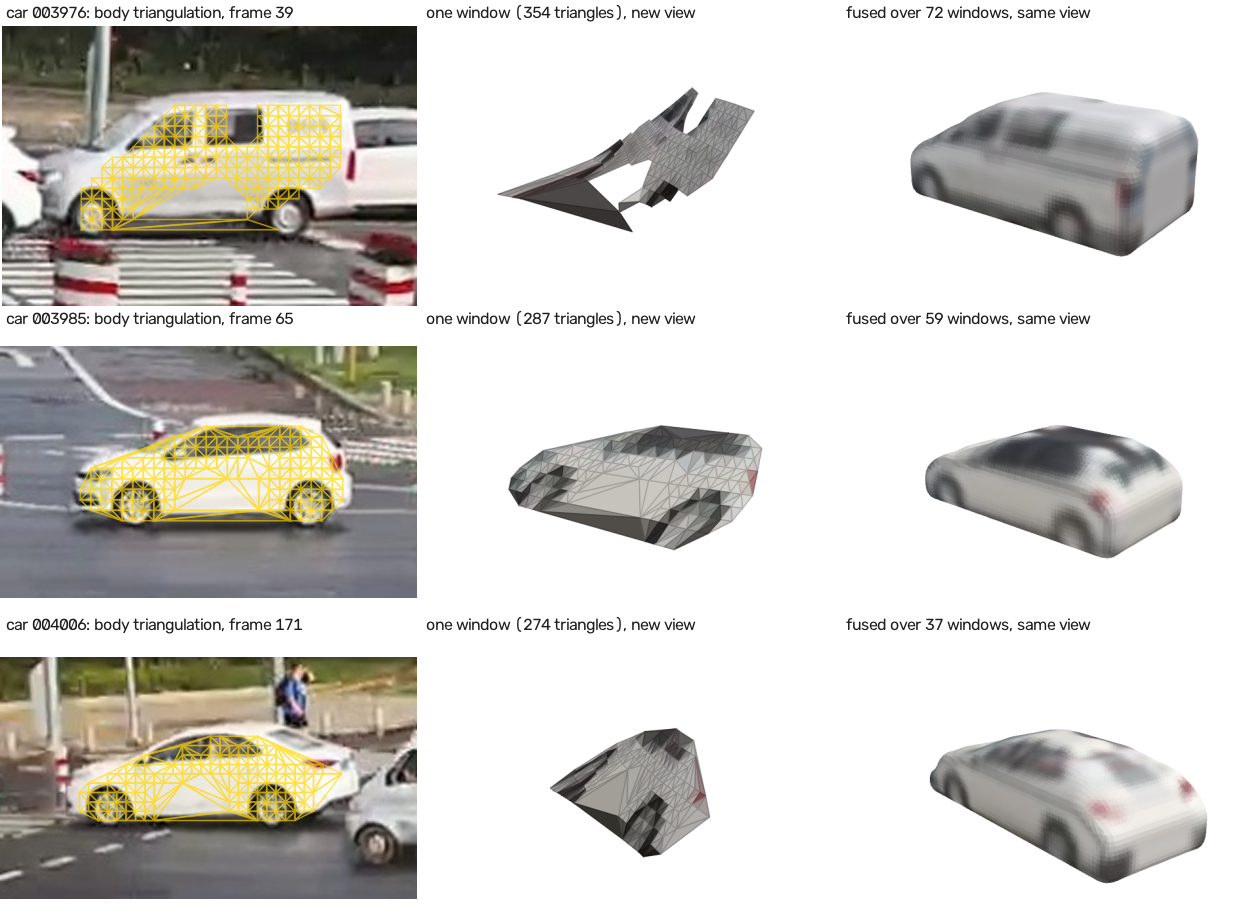
\includegraphics[width=\textwidth]{method_steps.png}
\caption{From triangulation to model, three cars of intersection A. Left: the body triangulation in one frame.
Middle: the same triangles in 3D after the window's joint solve, from a new viewpoint --- one window is noisy along
the viewing rays. Right: the model fused over all windows of the car (one rigid car, symmetry, weighted-median height
field, cabin from silhouettes, Poisson surface, video colours), from the same viewpoint.}
\label{fig:steps}
\end{figure}

\begin{figure}[t]
\centering
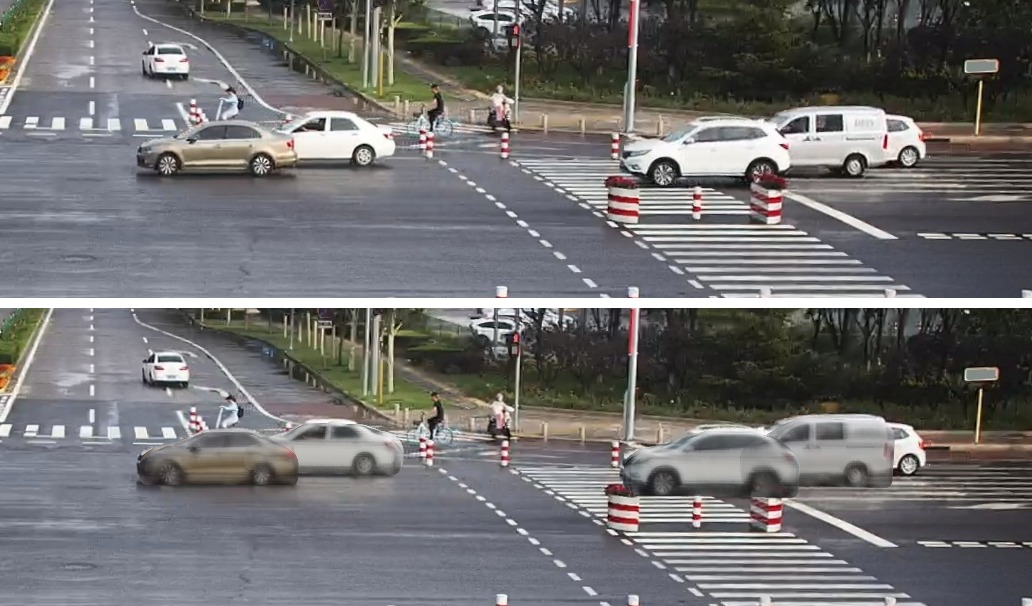
\includegraphics[width=\textwidth]{scene_models.jpg}
\caption{Intersection A, frame 30, about 60--70~m from the camera. Top: the video. Bottom: the four car models,
fused over the whole video, drawn at their pose in this frame (all models whose projection matches the car's
silhouette in this frame).}
\label{fig:scene}
\end{figure}

\begin{figure}[t]
\centering
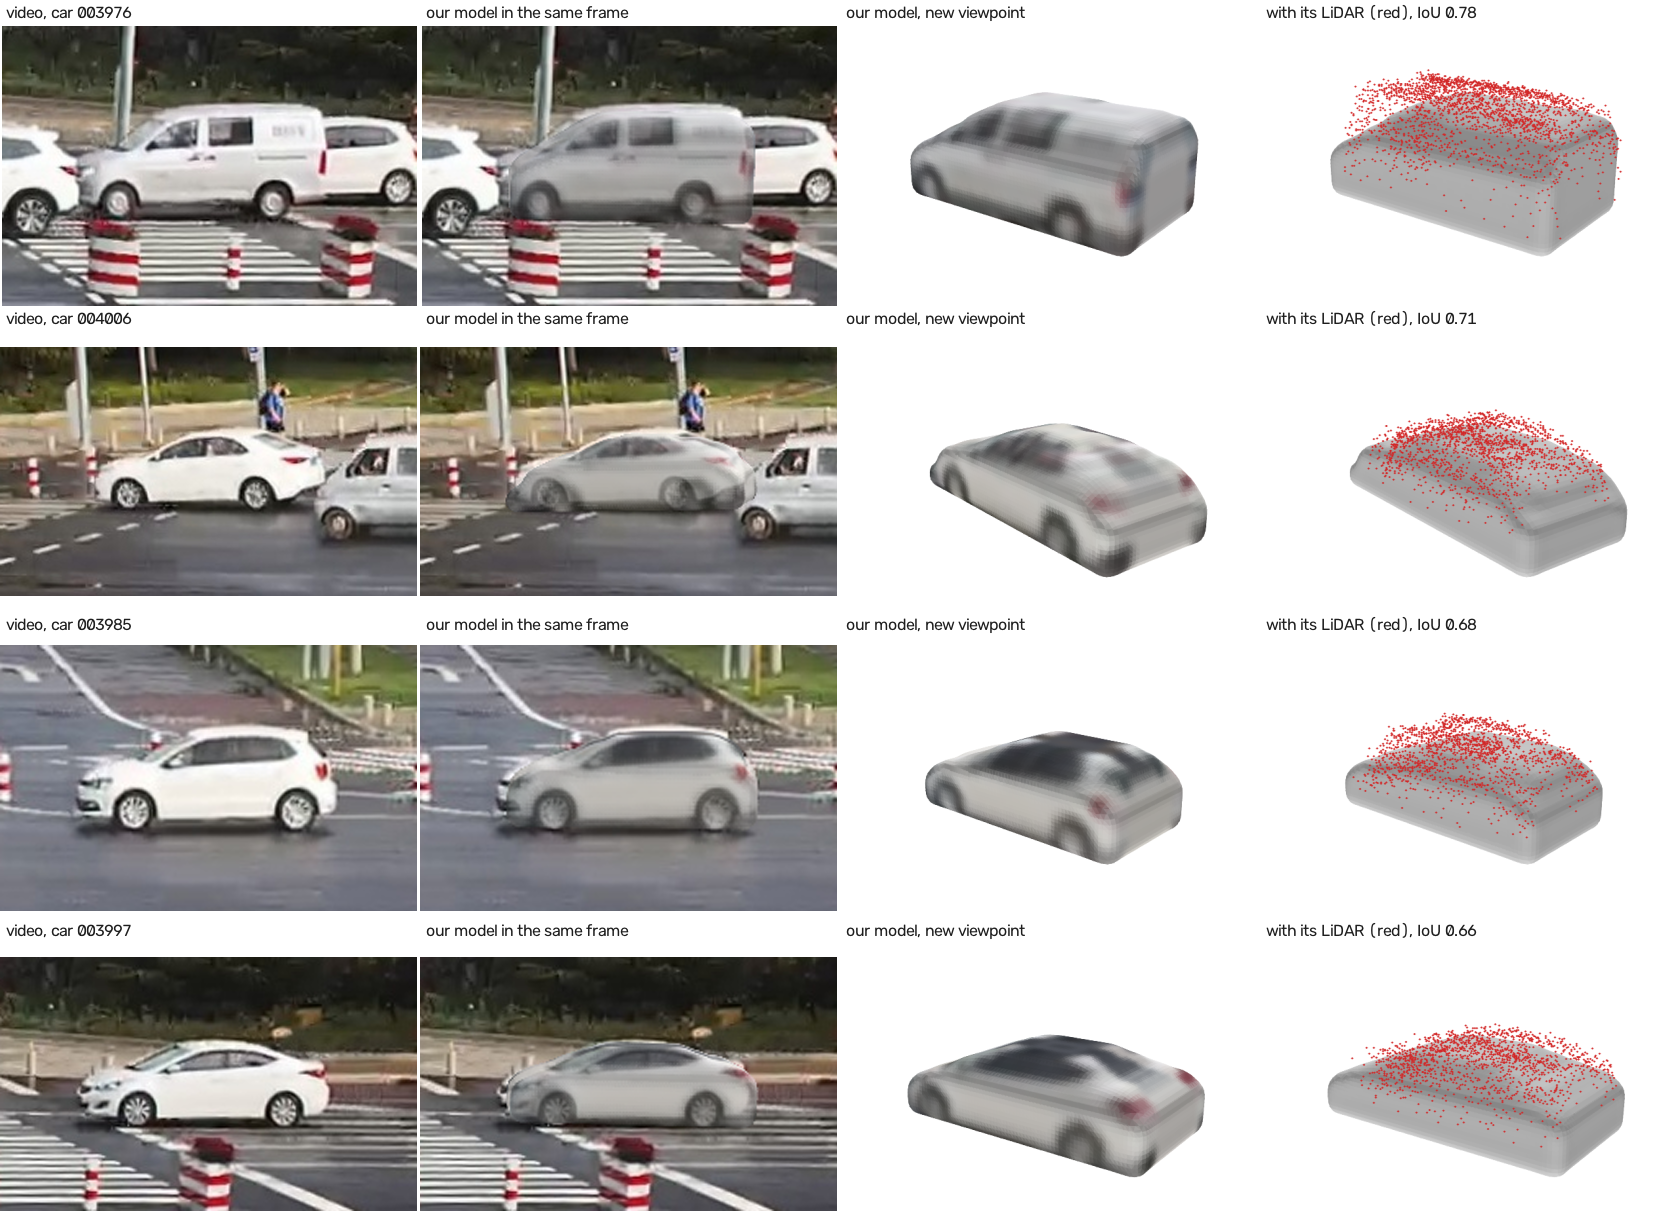
\includegraphics[width=\textwidth]{cars_best.png}
\caption{Four best-reconstructed cars of intersection A. A van, a hatchback and two sedans, each shown in the frame
where it is largest and unoccluded. Left to right: the video; our model drawn into the same frame; the model from a
new viewpoint, with the colours of the video pixels; the model with the car's accumulated LiDAR (red, evaluation
only) and the solid IoU against it.}
\label{fig:cars}
\end{figure}
\begin{table}[t]
\centering
\caption{Ablation on both intersections, changes added one at a time. IoU and height error against the gap-closed LiDAR; $|\Delta L|$, $|\Delta H|$: mean size errors (m); on the cars evaluated in every row (17 on A, 7 on B). The pipeline is deterministic: repeated runs give identical numbers.}
\label{tab:ablation}
\setlength{\tabcolsep}{3.5pt}
\resizebox{\textwidth}{!}{%
\begin{tabular}{lcccccccc}
\toprule
 & \multicolumn{4}{c}{intersection A} & \multicolumn{4}{c}{B (not used for tuning)} \\
\cmidrule(lr){2-5}\cmidrule(lr){6-9}
 & IoU & h.~err & $|\Delta L|$ & $|\Delta H|$ & IoU & h.~err & $|\Delta L|$ & $|\Delta H|$ \\
\midrule
previous version & 0.564 & 24.8 & 0.70 & 0.31 & 0.392 & 24.6 & 2.33 & 0.26 \\
+ cabin taper & 0.567 & 24.5 & 0.70 & 0.31 & 0.393 & 24.6 & 2.33 & 0.26 \\
+ length prior where never seen side-on & 0.580 & 24.5 & 0.48 & 0.31 & 0.486 & 26.3 & 0.29 & 0.21 \\
+ one rigid car per track & 0.599 & 23.1 & 0.45 & 0.32 & 0.524 & 26.4 & 0.25 & 0.16 \\
+ softer hull vote for those cars & 0.608 & 22.6 & 0.45 & 0.33 & 0.564 & 25.0 & 0.25 & 0.18 \\
+ body-type profile for them (ours) & \textbf{0.615} & 20.5 & 0.45 & 0.31 & \textbf{0.571} & 26.6 & 0.25 & 0.15 \\
\bottomrule
\end{tabular}}
\end{table}


\paragraph{Ablation.} Table~\ref{tab:ablation} adds the changes one at a time to the previous version of the method,
on the same windows; the pipeline is deterministic, and repeated runs, with the track solves recomputed from
scratch, give identical numbers.
The taper of the cabin --- above the belt line the roof is narrowed to about 72\,\% of the body width, as a car's
cabin is --- changes the IoU little but keeps the glass off the roof edges. The length prior for the cars no window
saw side-on is the largest single step on B ($+0.093$), where it cuts the length error from 2.3 to 0.3~m, and gains
$+0.013$ on A. Applied to every car, the cap scores a little higher on A but cuts the measured vans\footnote{In an
earlier version of the method, capping every car at 4.6~m gave 0.598 on A against 0.590 for capping only the cars
never seen side-on, and 0.579 against 0.583 on 84 cars of A, B and five clips of the larger evaluation; on the 18
vehicles longer than 4.7~m among them it gave 0.543, against 0.574 without a cap and 0.580 with the conditional
cap.}.
Solving the windows of a car together, as one rigid car, gains $+0.019$ on A and $+0.038$ on B. The softer hull vote
for the prior cars gives back the volume the strict vote cut away ($+0.009$ and $+0.040$), and the body-type profile
for those cars adds $+0.007$ on both; it lowers the height error on A (22.6 to 20.5~cm) but not on B (25.0 to
26.6~cm), where only the overall height improves ($|\Delta H|$ 0.18 to 0.15~m). We also tried and dropped, because they did not
help on A and B: a weight of each window by its triangulation angle; a term making the points of one physical
location in two windows coincide (it brings them together, from 0.5--0.8~m apart to 2~cm, but the shape does not
improve); the body height as a soft penalty instead of a bound; a texture test against shadows on dark cars; and a
Poisson surface \cite{kazhdan2006} of the windows' oriented points in place of the median height field, which keeps
whatever a minority of windows sees, a neighbouring car included.

\paragraph{Intersection B.} The same method reaches \BsixClosed{} against \BlabClosed{} for the
labelled boxes (Table~\ref{tab:main}). B is harder than A: most cars drive away from the camera and are seen only
from behind (Fig.~\ref{fig:trianB}). The textured part is then the rear, whose depth is measured along the viewing
ray, and the silhouette cone is long in the same direction: before the length prior, these cars came out too long
and too narrow (previous version: \BprevClosed{}). No window of them is side-on, so their length and profile come from
the body type --- a prior, not a measurement; with it our models are level with the labelled boxes on these cars
(Table~\ref{tab:paired}: $+0.024$, the interval contains zero); with seven cars this is a preliminary result. The car centres are less accurate than on A (median error \Bcentre{}~m against \Acentre{}~m), because the
visible rear is two metres from the centre: with the 3~m matching gate only one car is matched, and we use 5~m on
B.

\begin{figure}[t]
\centering
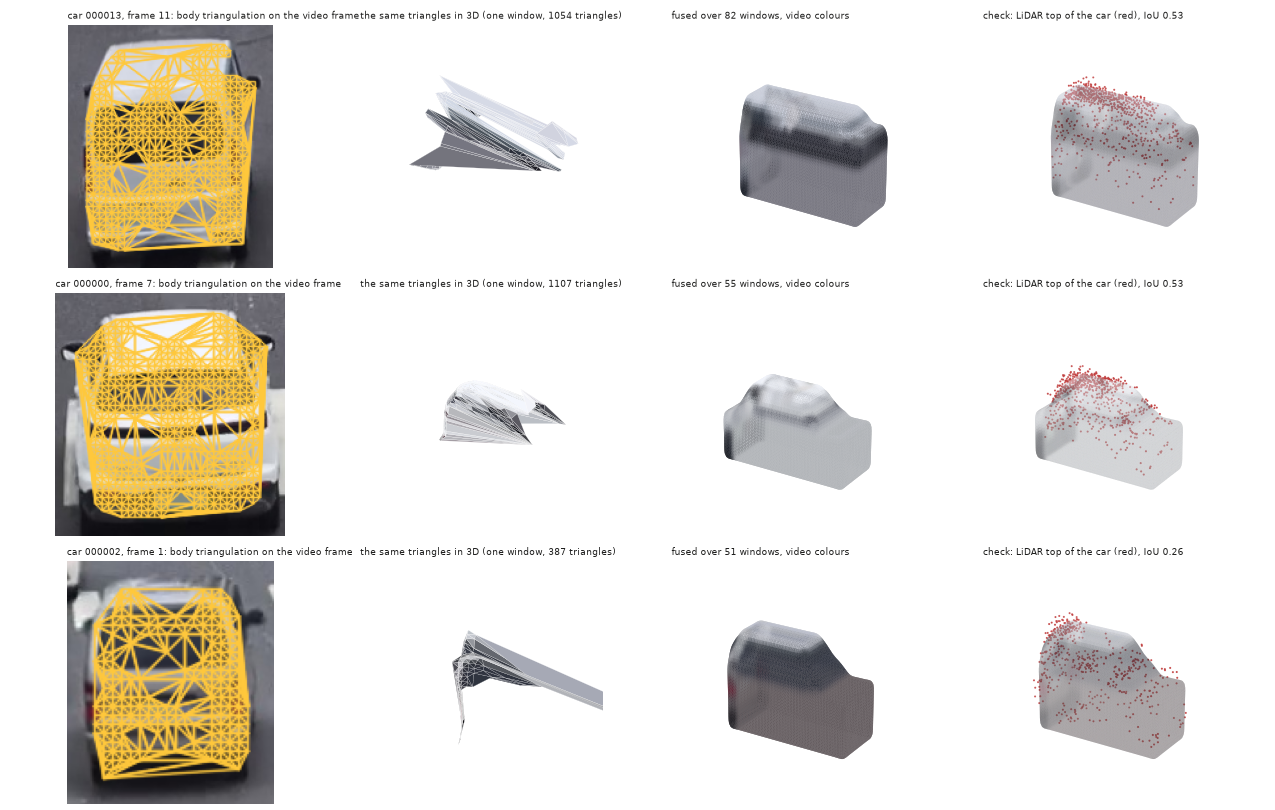
\includegraphics[width=\textwidth]{triangulation_B.png}
\caption{Intersection B (DAIR-V2X-C), cars seen from behind. The rear is triangulated well, but the side is never seen
and the silhouette cone is long along the viewing ray: without a prior the models come out too long and too narrow.
Their length and profile therefore come from the body type.}
\label{fig:trianB}
\end{figure}

\begin{table}[!htb]
\centering
\caption{Larger evaluation, no parameter changed: clips of DAIR-V2X-C and sequences of V2X-Seq-SPD, two or three per intersection. Mean solid IoU of our models and of the labelled boxes against the cars' raw and gap-closed accumulated LiDAR; median position error of our models along and across the viewing ray.}
\label{tab:large}
\footnotesize
\begin{tabular}{llrcccccc}
\toprule
Dataset & Intersection & Cars & \multicolumn{2}{c}{raw LiDAR} & \multicolumn{2}{c}{closed LiDAR} & \multicolumn{2}{c}{position (m)} \\
\cmidrule(lr){4-5}\cmidrule(lr){6-7}\cmidrule(lr){8-9}
 & & & ours & box & ours & box & along & across \\
\midrule
DAIR-V2X-C & yz02 & 17 & 0.478 & 0.451 & 0.652 & 0.631 & 1.87 & 0.82 \\
 & yz06 & 33 & 0.482 & 0.509 & 0.617 & 0.638 & 1.63 & 0.57 \\
 & yz08 & 5 & 0.448 & 0.499 & 0.612 & 0.635 & 1.24 & 0.35 \\
 & yz09 & 23 & 0.468 & 0.474 & 0.620 & 0.630 & 0.85 & 0.83 \\
 & yz10 & 8 & 0.465 & 0.422 & 0.623 & 0.606 & 2.03 & 0.57 \\
 & yz13 & 6 & 0.550 & 0.551 & 0.636 & 0.666 & 1.32 & 0.38 \\
 & yz16 & 17 & 0.379 & 0.363 & 0.541 & 0.536 & 1.07 & 0.38 \\
 & \textbf{all} & \textbf{109} & \textbf{0.463} & \textbf{0.465} & \textbf{0.612} & \textbf{0.618} & \textbf{1.44} & \textbf{0.59} \\
\midrule
V2X-Seq-SPD & yz06 & 45 & 0.517 & 0.571 & 0.663 & 0.688 & 1.51 & 0.32 \\
 & yz08 & 10 & 0.344 & 0.393 & 0.540 & 0.571 & 2.05 & 0.15 \\
 & yz09 & 16 & 0.431 & 0.466 & 0.628 & 0.653 & 0.76 & 0.33 \\
 & yz10 & 7 & 0.323 & 0.342 & 0.527 & 0.574 & 2.21 & 0.22 \\
 & yz13 & 13 & 0.517 & 0.531 & 0.635 & 0.611 & 2.35 & 0.29 \\
 & yz16 & 13 & 0.322 & 0.339 & 0.542 & 0.544 & 1.04 & 0.33 \\
 & \textbf{all} & \textbf{104} & \textbf{0.450} & \textbf{0.488} & \textbf{0.618} & \textbf{0.636} & \textbf{1.37} & \textbf{0.29} \\
\bottomrule
\end{tabular}
\end{table}


\paragraph{Thirteen intersections, two datasets.} To test the method beyond the two intersections it was developed on,
we ran it unchanged on \DairClips{} clips of DAIR-V2X-C (\DairFrames{} frames at \DairSites{} intersections) and on
\SpdClips{} sequences of the full V2X-Seq-SPD (\SpdFrames{} frames at \SpdSites{} intersections), two or three of the
longest per intersection, without intersection A; frames missing from the recording are skipped and the motion is
measured per time slot. Table~\ref{tab:large} scores every car with a LiDAR reference and a labelled box against both
references. On DAIR-V2X-C the \DairCars{} cars reach \DairOursClosed{} against \DairBoxClosed{} for the labelled boxes
on the closed reference and \DairOursRaw{} against \DairBoxRaw{} on the raw one; on V2X-Seq-SPD the \SpdCars{} cars
reach \SpdOursClosed{} against \SpdBoxClosed{} (\SpdOursRaw{} against \SpdBoxRaw{} raw). The paired differences are
not separated from zero (Table~\ref{tab:paired}), also on the clips that informed no design choice (71 cars of
DAIR-V2X-C, $+0.001$ $[-0.021, +0.022]$; 94 of V2X-Seq-SPD, $-0.017$ $[-0.042, +0.009]$). The previous version of the method was 0.080 and 0.118 below
the boxes on the same cars; the current one gains $+0.074$ $[+0.050, +0.099]$ and $+0.099$ $[+0.075, +0.124]$ over it.
The position along
the viewing ray (\DairAlong{}~m and \SpdAlong{}~m) remains the main error. Figure~\ref{fig:large} shows eight car
models of all datasets next to the cars in the video.

\begin{figure}[!htb]
\centering
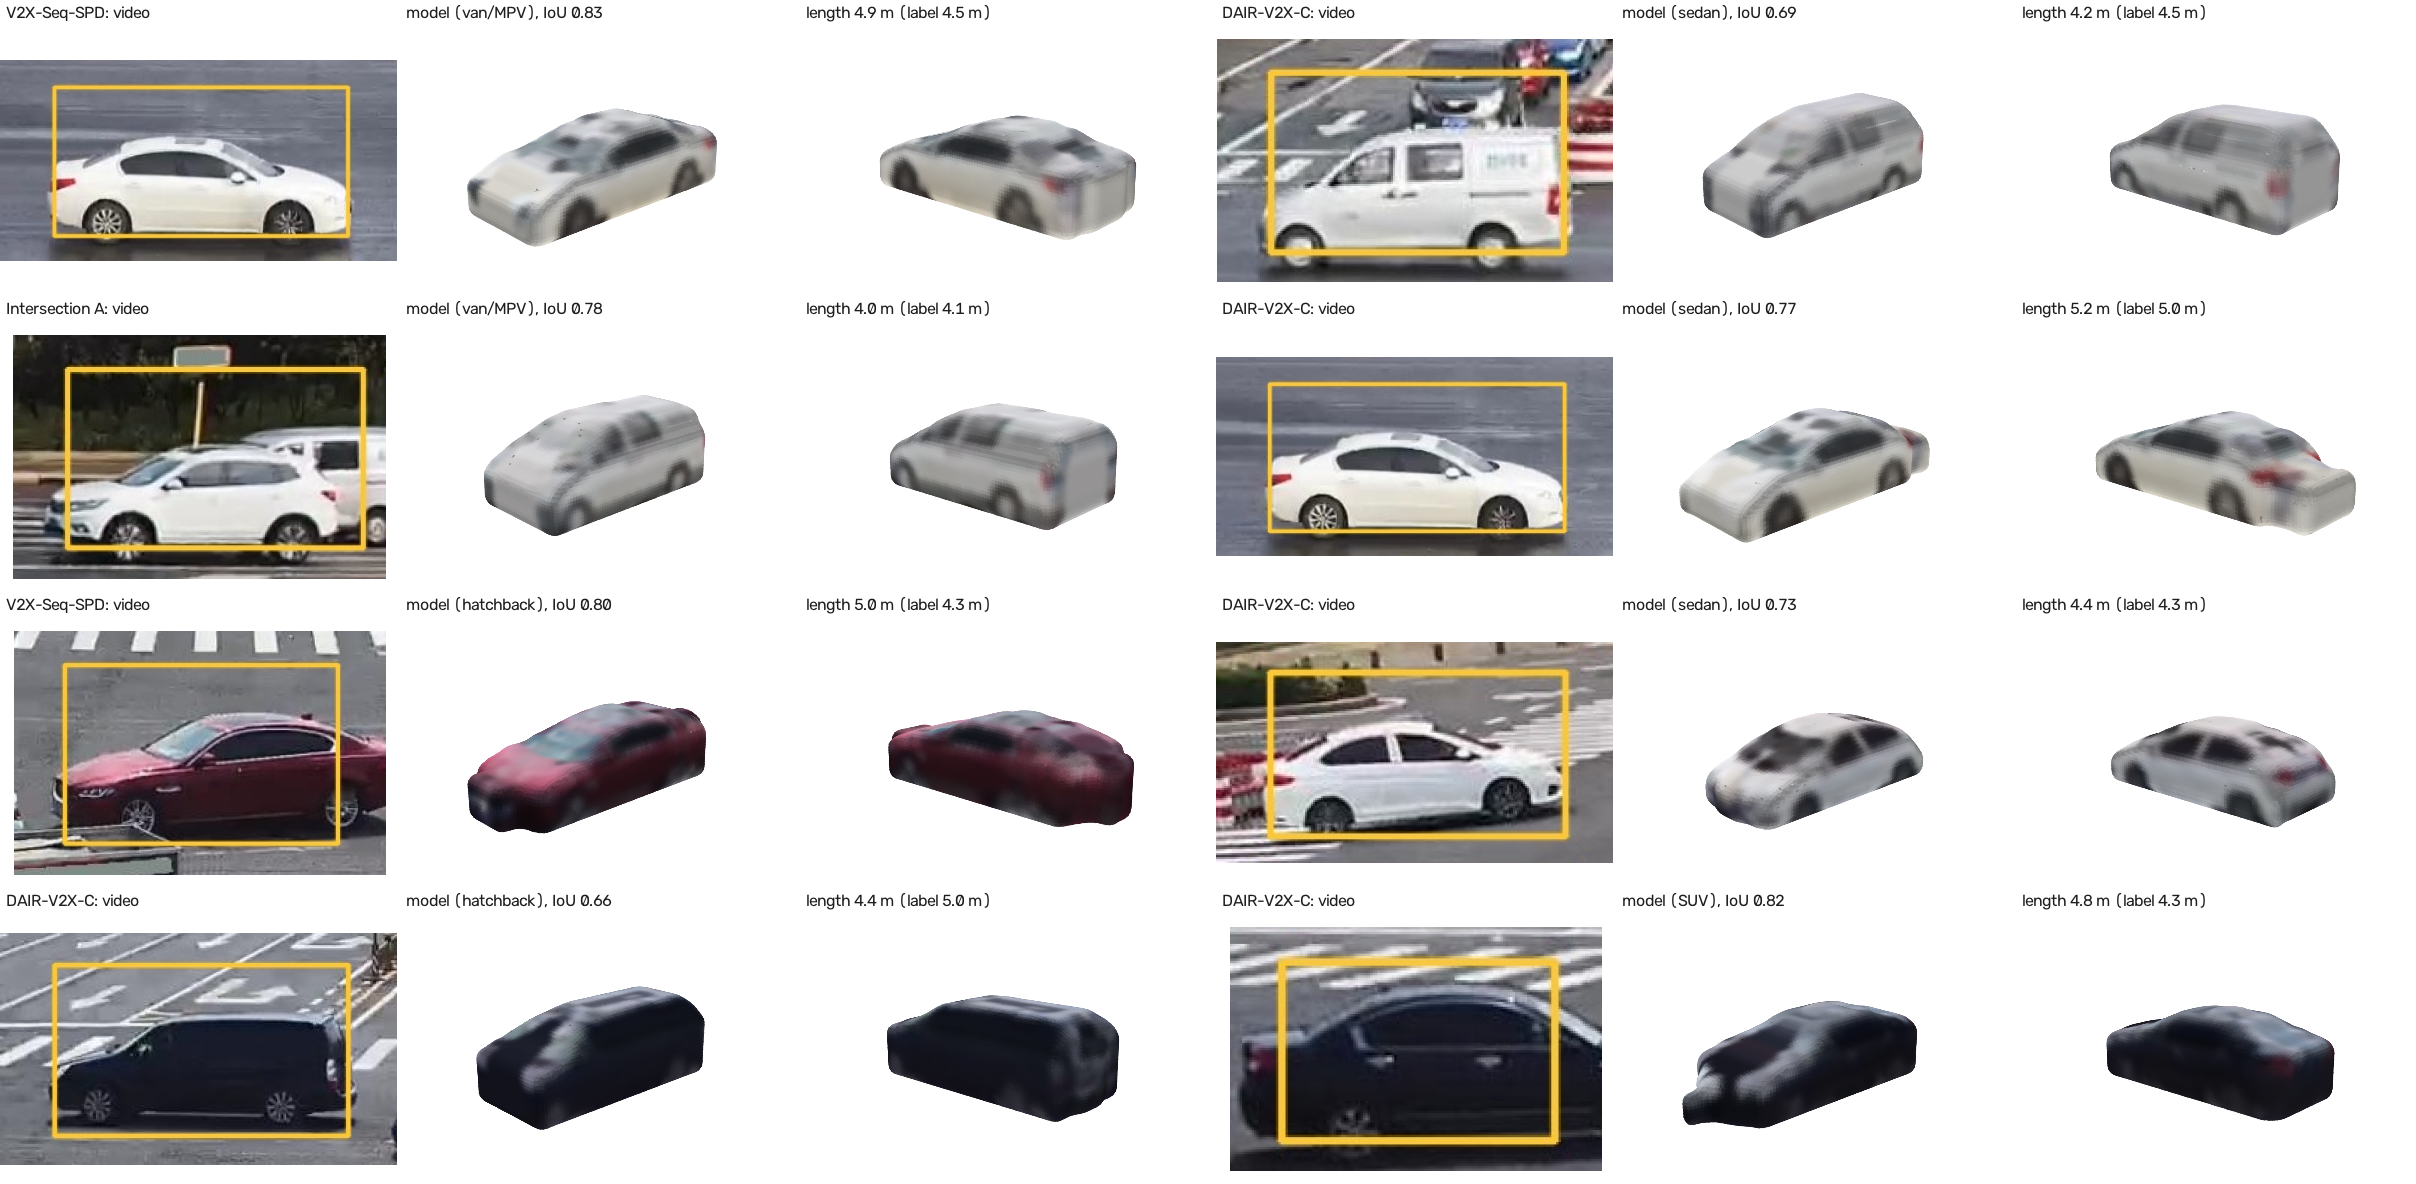
\includegraphics[width=\textwidth]{best_models.png}
\caption{Eight car models of all datasets, solved on the SAM masks and LiDAR-fitted cuboids. Per car: the video frame with
the car framed; the model with the original pixels of its best views from the front left and from the rear left; its
solid IoU against the closed LiDAR and its length against the labelled length.}
\label{fig:large}
\end{figure}

\paragraph{Pedestrians and cyclists.} A person or a cyclist is thin and partly non-rigid, and the rigid
triangulation finds few points on it. Its silhouette, however, is clear in most frames, and its bottom touches the
road, so we reconstruct it from the silhouettes alone: the ground point under the silhouette gives the path and the
direction of travel, and a symmetric visual hull in the object's own frame, with an elliptic horizontal section at
most 0.6~m wide, gives the shape. A wet road mirrors the object; the contact line is the first row about which the
image is mirror-symmetric. Each object is selected by its labelled 2D box in one frame. Of fourteen pedestrians,
cyclists and motorcyclists within 35~m of V2X-Seq-SPD, our own silhouette tracker gave usable models for two; the
others came out as fragments --- an umbrella, legs, a shirt, a bicycle frame --- because the background difference
loses dark clothes on dark asphalt and occluded parts. With the labelled 2D boxes as the tracker instead, everything
else unchanged, eight of the fourteen give a model and six none: their silhouettes do not agree on one shape, or no
frame shows them unoccluded. For the four in Fig.~\ref{fig:vru} whole figures appear, and the silhouette overlap on
frames left out of the carving rises from 0.20--0.46 to 0.45--0.64; over all eight it spans 0.02--0.64. The shape
step works where the object is followed whole; detection and tracking are the main limit. Three of the four figures
are 0.4 to 0.5~m too tall, as the silhouette cone rises toward the camera, and the thin parts of a bicycle are lost.

\begin{figure}[!htb]
\centering
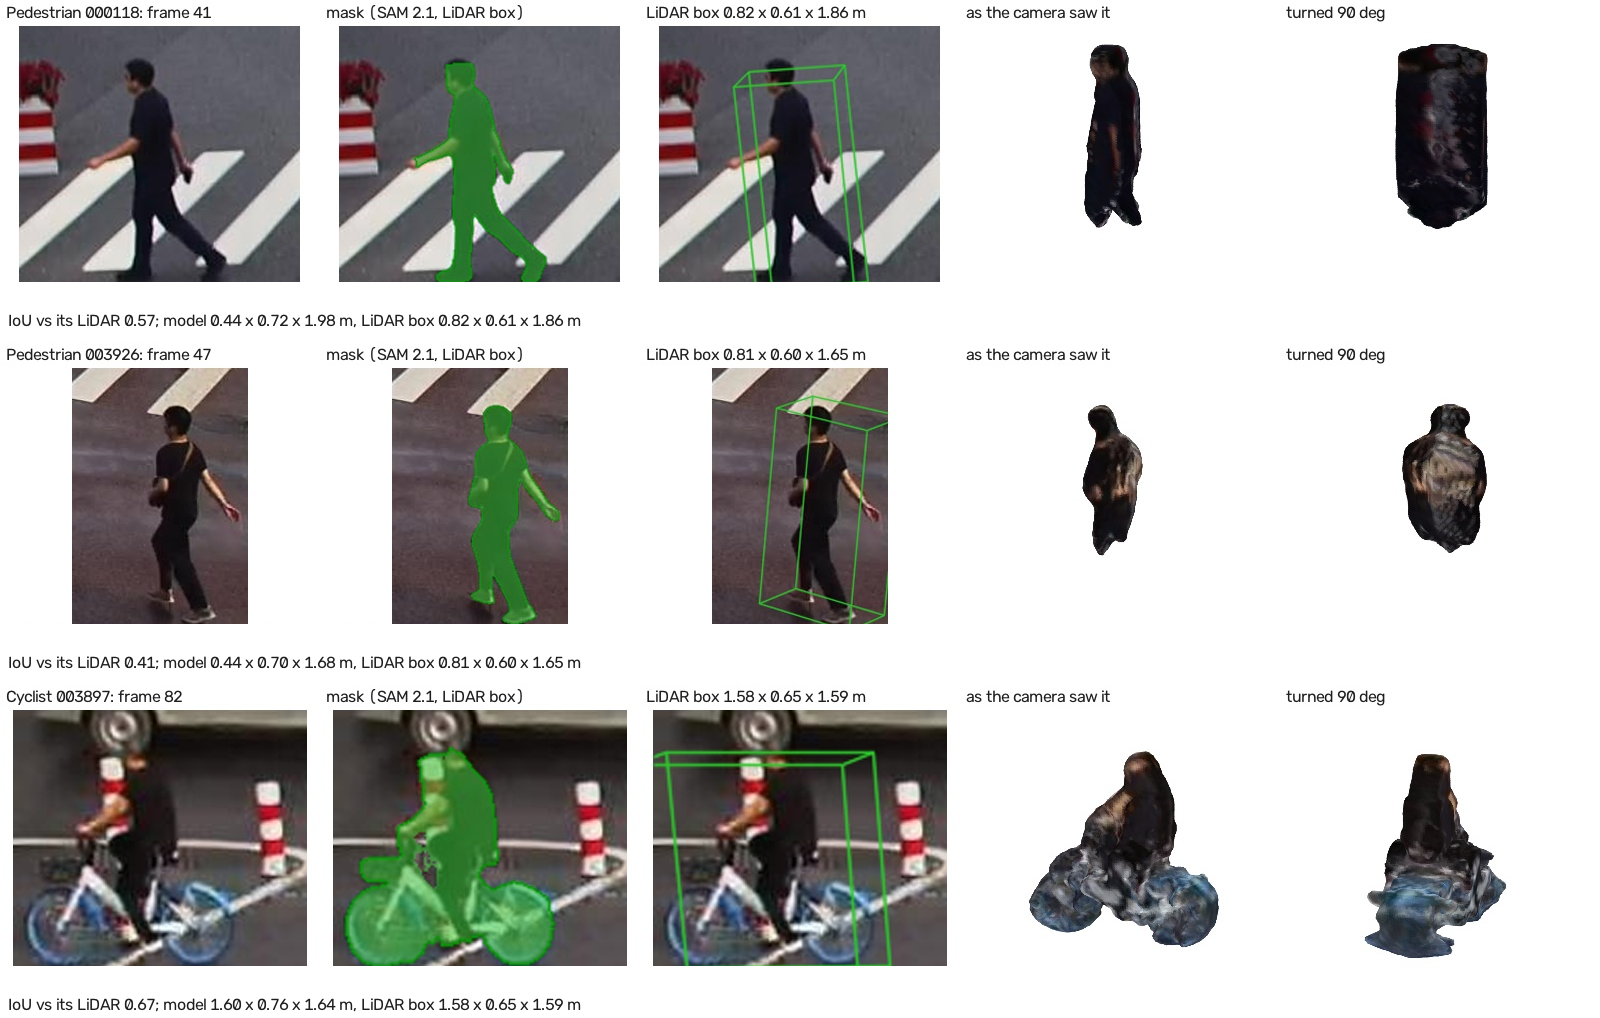
\includegraphics[width=0.85\textwidth]{vru_compare.png}
\caption{Pedestrians and cyclists of V2X-Seq-SPD from silhouettes, within 35~m. Per row: the video with the object
framed; the model with our own silhouette tracker; the model with the labelled 2D boxes as the tracker; the same from
the side, with its height against the labelled one. IoU: the model's silhouette against the observed one on the
frames left out of the carving.}
\label{fig:vru}
\end{figure}

With a good cuboid track and good masks the same carving gives a whole object. Fig.~\ref{fig:cyclist} shows a cyclist
of V2X-Seq-SPD (seq.~59) carved from 61 masks, with the cuboid track fitted to the cyclist's own LiDAR points and the
masks from a promptable segmenter (SAM~2.1) prompted by the labelled 2D box, as one example of how both can be
obtained. Along the line of sight the silhouettes cannot measure depth; there the carve is bounded by the camera-side
surface triangulated over the whole pass (rigid tracks, reprojection error at most 1~px) and mirrored about the
centre plane. Its top comes from the silhouettes. The model is 1.60$\times$0.78$\times$1.56~m against the LiDAR box's
1.63$\times$0.67$\times$1.50~m, solid IoU 0.64 against its accumulated LiDAR; the carve alone scores 0.64 too, with
40\,\% more volume. For this example the camera is the rigid
one that projects the road as the calibration does: the calibration's rotation of these sequences is not orthonormal
(the row of the image's vertical has norm 0.83) and projects every height about 17\% short.

\begin{figure}[!htb]
\centering
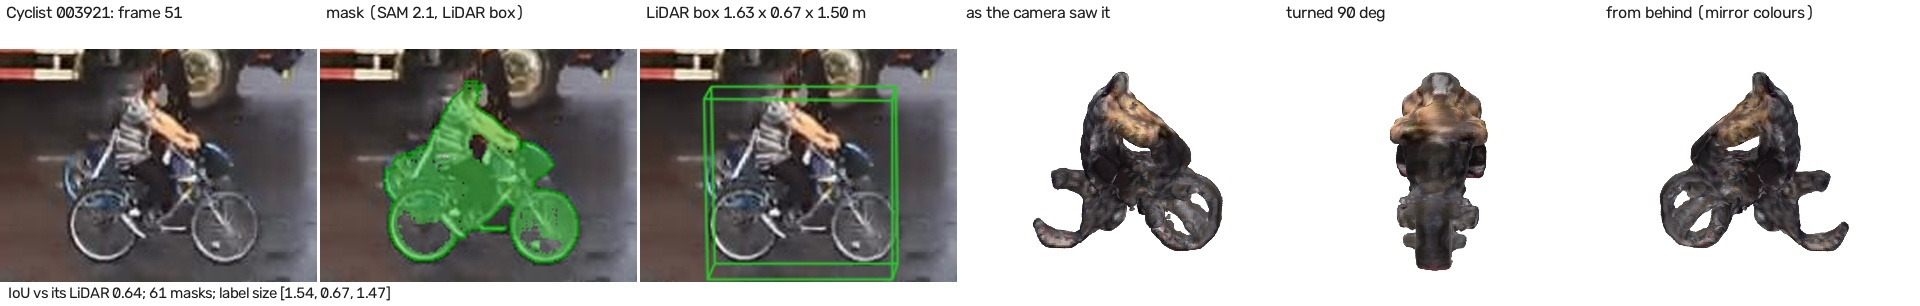
\includegraphics[width=\textwidth]{vru_cyclist.jpg}
\caption{A cyclist of V2X-Seq-SPD carved from its masks and bounded by its triangulated surface. From the left: a frame of the video; its mask; the cuboid
fitted to the cyclist's LiDAR; the model as the camera saw it, turned by 90$^\circ$ and from behind (the unseen side
coloured by mirroring).}
\label{fig:cyclist}
\end{figure}

\paragraph{A moving camera.} To test the dependence on the fixed camera we ran the pipeline on the vehicle side of the
same sequence. The camera's pose comes from monocular visual odometry: corners tracked frame to frame, the five-point
essential matrix \cite{nister5pt} for the rotation and the direction of the step, and the step's length from the road
plane, whose homography between two frames is linear in the length for a camera of known height \cite{songchandraker}.
The background of a frame is the median of its neighbours warped onto it through the road plane, and a blob is moving
when its flow differs from the flow it would have standing still on the road. The odometry is accurate enough (yaw
error $0.06^\circ$ per frame, \Egopath{} too long over 138~m), but of \Egolabels{} moving labelled cars within 40~m only
\Egofound{} are found (recall \Egorecall{}, precision \Egoprecision{}) and no track lasts the five windows a model
needs (Fig.~\ref{fig:ego}). In three test frames the GPS/INS poses instead of the odometry gave no better result, which
indicates that the viewpoint, not the odometry, is the limiting factor. From 1.7~m the road-contact anchor gives a weak depth beyond 20~m, the warped background aligns only the
road, and the cars ahead are seen from behind for the whole sequence.

\begin{figure}[t]
\centering
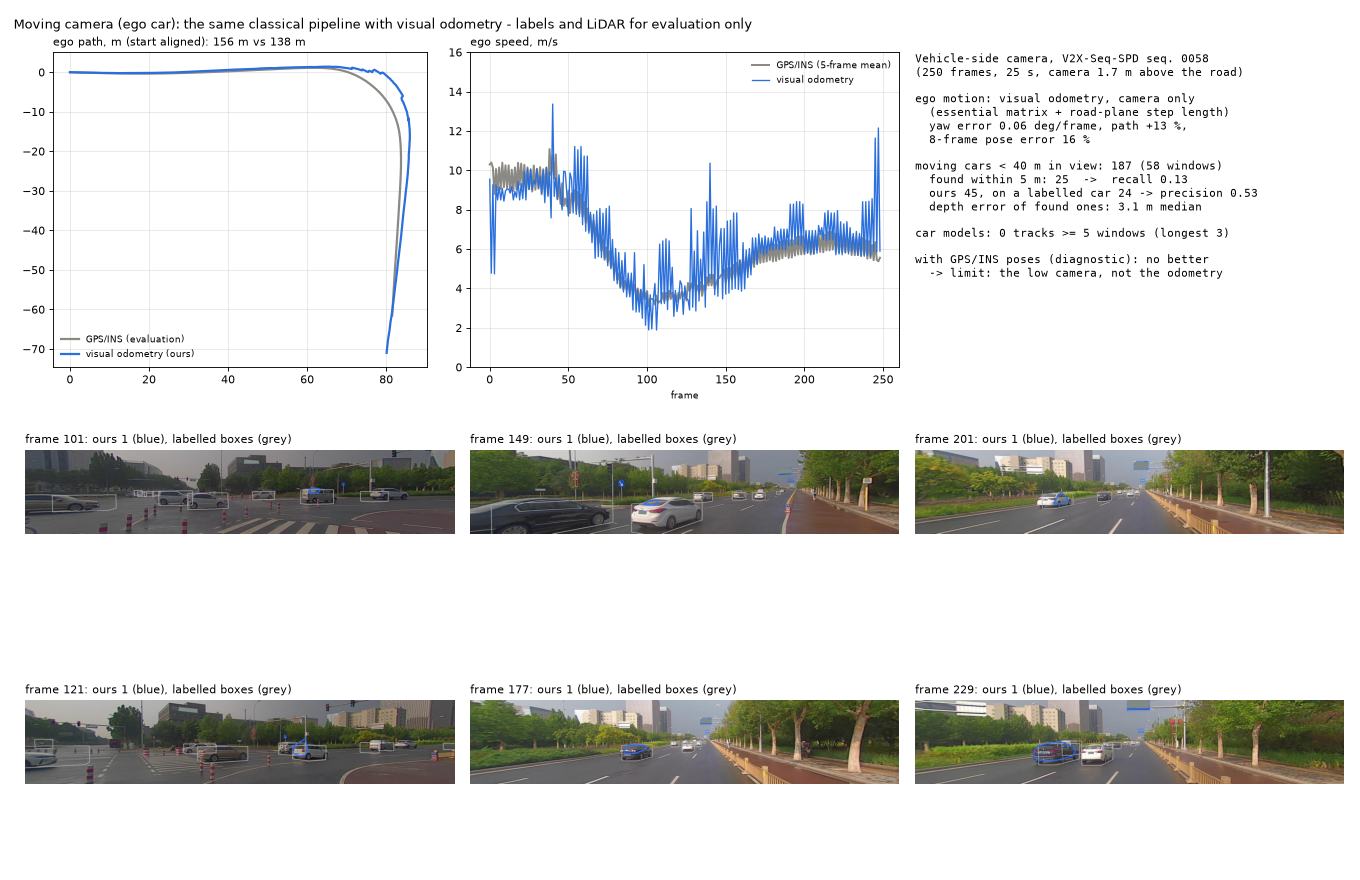
\includegraphics[width=\textwidth]{moving_camera.png}
\caption{The pipeline on a moving vehicle camera (V2X-Seq vehicle side). Top: the ego path and speed from visual
odometry against GPS/INS (evaluation only). Bottom: our detections (blue) and the labelled boxes (grey). Few cars are
found; the method needs the fixed, elevated camera.}
\label{fig:ego}
\end{figure}

% ------------------------------------------------------------------------------------------------------------------
\section{Comparison with Other Approaches}\label{sec:comparison}

There is no common benchmark for car \emph{shapes} from roadside video, and published monocular detectors report the
average precision of boxes, not shape IoU against LiDAR; their numbers are not comparable with ours, and we did not
retrain them. Table~\ref{tab:compare} therefore compares what each family of methods needs and produces.
Quantitatively, the labelled box and the box of our own size in Table~\ref{tab:main} stand in for a perfect and for a
size-only box detector: our shapes exceed the latter on A and B and are level with the former on the larger
evaluation (Tables~\ref{tab:large} and~\ref{tab:paired}).

\begin{table}[t]
\centering
\caption{What families of methods need and produce. ``3D labels'': labelled 3D boxes or shapes for training.}
\label{tab:compare}
\setlength{\tabcolsep}{3pt}
\footnotesize
\newcolumntype{L}[1]{>{\raggedright\arraybackslash}p{#1}}
\begin{tabular}{L{3.7cm}L{1.5cm}L{1.6cm}L{1.4cm}L{3.0cm}}
\toprule
family & training data & input & output & main limitation here \\
\midrule
learned box detectors \cite{smoke,monodle,monoflex,fcos3d} & 3D labels & one image & 3D box & no shape; trained per camera type \\
learned roadside detectors \cite{bevheight} & 3D labels & one image & 3D box & no shape; needs roadside labels \\
geometric box lifting \cite{deep3dbox,lift,efficient_orig} & 2D labels or none & one image & 3D box & size prior, no shape \\
learned shape models \cite{kar2015,deepmanta,rcnn3d} & CAD / 3D shapes & one image & shape & shape prior; not shown at 60~m \\
visual hull, space carving \cite{laurentini,spacecarving} & none & many cameras & shape & needs widely spread views \\
multibody SfM \cite{ozden2010,kumar2017} & none & video & points / depth & sparse, no closed shape \\
\textbf{ours} & none & video of a fixed camera & closed shape & needs motion; fails end-on \\
\bottomrule
\end{tabular}
\end{table}


Learned box detectors \cite{smoke,monodle,bevheight} are fast and robust at short and medium range but need
thousands of labelled boxes from comparable cameras and output no shape. Learned shape models
\cite{kar2015,deepmanta,rcnn3d} produce shapes from a single image but need a shape prior learned from CAD models or
3D annotations, and they have not been evaluated at 60~m from a roadside camera. Silhouette methods
\cite{laurentini,spacecarving} need many, widely spread viewpoints; a single high camera gives a narrow range of
directions per car, which is why our visual hull alone over-estimates the height and the length of cars seen end-on.
Our method uses the motion of the car itself to obtain the views that a static multi-camera setup would provide, and
uses the textured body for depth where silhouettes are ambiguous; it needs no training data, but it needs a fixed,
calibrated camera and enough motion, and it reconstructs a car only after it has been tracked for about two seconds.

% ------------------------------------------------------------------------------------------------------------------
\section{Limitations}\label{sec:limits}

\begin{itemize}
\item \emph{Coverage.} Of the moving vehicles the camera sees, about half on intersection A and a quarter on B get a
  model. Most of the others are never found by the window stage (beyond about 80~m, or merged with a neighbour in the
  foreground) or are tracked for fewer than five windows; stopped cars have no parallax and are not reconstructed.
\item \emph{Position along the viewing ray.} A single camera places the car about a metre off along the ray
  (Sect.~\ref{sec:results}); the shape is not affected, the position is.
\item \emph{Priors.} A car never seen side-on --- typically one seen only from behind --- takes the length and the
  profile of its body type; these cars are reported separately, and their score reflects the prior, not a measurement.
  The measured cars of V2X-Seq-SPD stay $0.05$ below their labelled boxes.
\item \emph{Tracks.} A track that switches to a neighbouring car for a few windows mixes the two into one model.
\item \emph{Tuning.} The parameters were chosen on the \Alabels{} cars of intersection A; B and five clips of the
  larger evaluation informed three choices (Sect.~\ref{sec:protocol}), and the clips that informed none give the same
  result. All intersections are in one city and use the same kind of camera.
\item \emph{Pedestrians and cyclists} need a good silhouette tracker: with ours most of them come out as fragments,
  with given 2D boxes eight of fourteen give a model, mostly whole figures but up to 0.5~m too tall, and thin parts
  are lost.
\item \emph{Viewpoint.} A moving, low camera fails (Sect.~\ref{sec:results}).
\item \emph{Run time.} The reference Python implementation needs one to two minutes per window on a single CPU core and a
  few minutes per car for the track solve; it is not optimised.
\end{itemize}

% ------------------------------------------------------------------------------------------------------------------
\section{Conclusion}

From a single fixed roadside camera, without any learning and without labels, the 3D shapes of the passing cars can
be recovered: measured against the cars' own LiDAR at up to 70~m, they are level with the labelled 3D boxes on
\DairCars{} and \SpdCars{} cars of two datasets and thirteen intersections and above them on the intersection the method
was developed on. Three ingredients carry it: the car's own motion, which turns one camera into many views of the
textured body; the whole video, solved as one rigid car and completed by symmetry and by silhouettes; and, only where
the video never measured the length, the body type. The same evaluation shows that the raw accumulated LiDAR is a
biased reference at long range and should be closed before it is used to compare shapes. What remains is less the
shape than finding and following the objects: half of the visible cars, and most pedestrians and cyclists, are lost
before reconstruction. Using learned detectors for detection and tracking while keeping the geometric reconstruction
is the natural next step.

\bibliographystyle{splncs04}
\bibliography{references}

\end{document}
